\chapter{Appendix - Introduktion}
I appendix A ges först en ordlista för arbetet och därefter beskrivs användarstudien av OpenTA. Resultatet och dess analys stod till grund för riktningen av arbetet som helhet. 

\section{Ordlista}
\label{app:ordlista}
\begin{labeling}{Bayesianska neurala nätverk}
\item [Aktiveringsfunktion]	Activation function
\item [Bakåtpropagation]	Back propagation
\item [Baslinje]	Baseline
\item [Bayesiansk djupinlärning]	Bayesian deep learning
\item [Bayesianska neurala nätverk]	Bayesian neural networks
\item [Binär entropi]	Binary crossentropy
\item [Binär klassificering]	Binary classification
\item [Datagraf]	Data Graph
\item [Direkt återkoppling]	Immediate feedback
\item [Djupinlärning]	Deep learning
\item [Edtech-industri]	Educational Technology
\item [Egenskaper]	Features
\item [Ett-noll-kodning]	One-hot encoding 
\item [Flerklass-klassificering]	Multiclass classification
\item [Framsida]	Front end
\item [Frågespråk]	Query Language
\item [Förlustfunktion]	Loss function
\item [Förskjutningsvärde]	Bias
\item [k-faldig korsvalidering]	k-fold cross validation
\item [Kategorisk entropi]	Categorical crossentropy
\item [Kvadratisk förlustfunktion]	Mean squared error
\item [Långt-korttidsminnesnätverk]	Long short-term memory
\item [Läsperiod]   En period på 8 veckor som avslutas med en tentamensvecka
\item [Läsvecka]    En vecka av en läsperiod
\item [Minimalt funktionell produkt]	Minimal Viable Product
\item [Multikorrelation]	Multi correlation
\item [Måldata]	Target data
\item [Optimeringsfunktion]	Optimizer
\item [Progressionsfält]	Progression bars
\item [Serversida]	Back end/Server side
\item [Skalär regression]	Scalar regression
\item [Slutpunkter]	Endpoints
\item [Stora öppna onlinekurser]	Massive Open Online Courses
\item [Tentamen]    Ett formellt prov för att examinera studenters kunskaper i slutet av en kurs
\item [Tentamensvecka]  En vecka i slutet av varje läsperiod avsedd för att skriva tentamen
\item [Tillplattningslager]	Flattening-layer
\item [Träffsäkerhet]	Accuracy
\item [Träningsdata]	Training data
\item [Tätt lager]	Dense layer
\item [Utsläckning]	Dropout
\item [Valideringsdata]	Validation data
\item [Viktregularisation]	Weight regularization
\item [Överanpassning]	Overfitting
\item [Övervakad inlärning]	Supervised learning
\end{labeling}
\newpage

\section{Användarstudie av OpenTA i kurs FFM234}
\label{app:opentasurvey}

%nämnd i kapitel \ref{sec: webb}

Här nedan beskrivs användarstudien av OpenTA i kurs FFM234 samt dess resultat. Användarenkäten har delats upp i frågor tillsammans med respektive frågas resultat som tillsammans utgör ett sammanställt dokument av användarstudien. Detta dokument presenteras nedan. 

%\begin{figure}[hbtp]
%    \centering
%    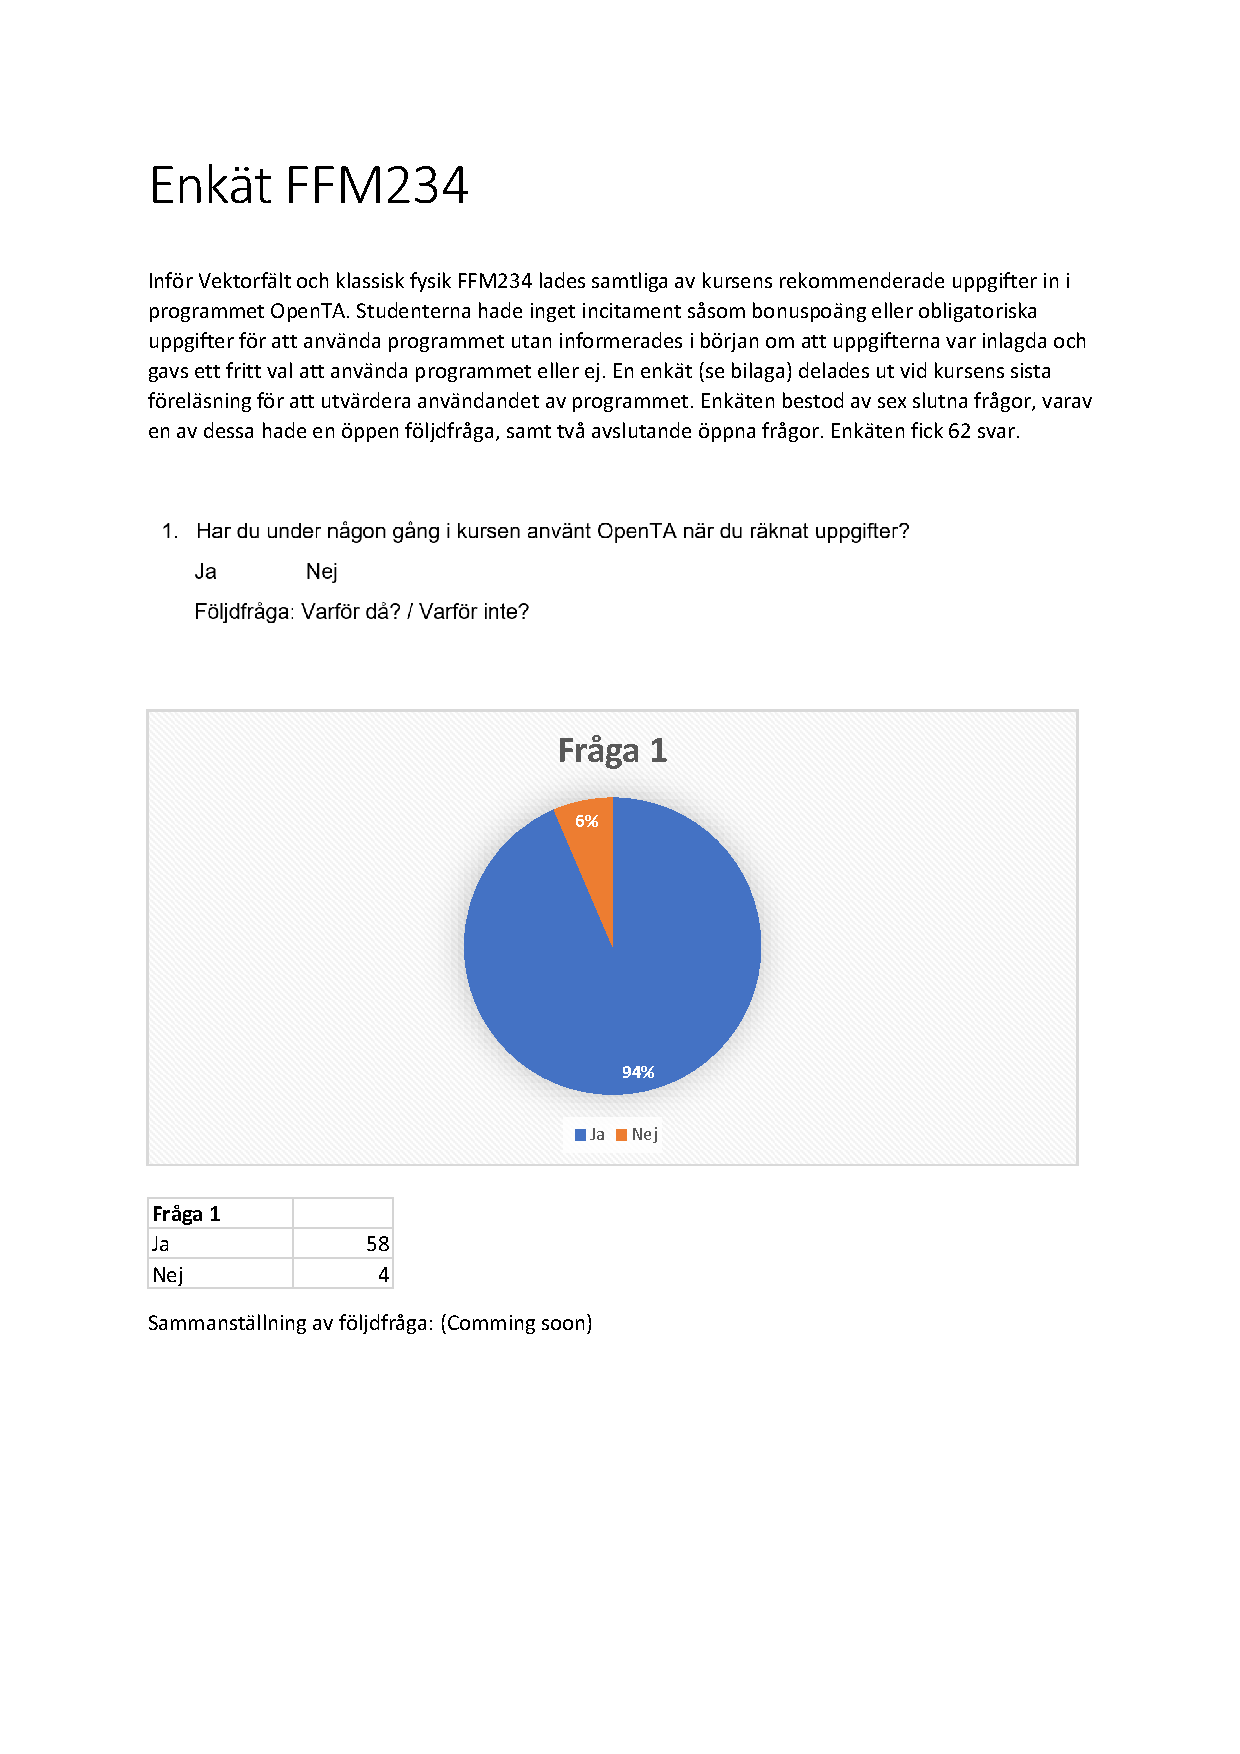
\includegraphics[page=1,scale=0.6]{appendix/form_survey.pdf}
%    \caption*{Brukarstudien med svarsstatistik, sida 1}
%    \label{fig:openform1}
%\end{figure}

%\begin{figure}%
%    \centering
%    \subfloat{{Sida 2}{\includegraphics[page=2,scale=0.55,angle=90]{appendix/form_survey.pdf}}}%
%    \qquad
%    \subfloat{{Sida 3}{\includegraphics[page=3,scale=0.55,angle=90]{appendix/form_survey.pdf} }}%
%    %\caption{2 Figures side by side}%
%    \label{fig:openform2-3}%
%\end{figure}

%\begin{figure}%
%    \centering
%    \subfloat{{Sida 4}{\includegraphics[page=4,scale=0.55,angle=90]{appendix/form_survey.pdf} }}%
%    \qquad
%   \subfloat{{Sida 5}{\includegraphics[page=5,scale=0.55,angle=90]{appendix/form_survey.pdf} }}%
%   %\caption{2 Figures side by side}%
%    \label{fig:openform4-5}%
%\end{figure}

\begin{figure}[hbtp]
    \centering
    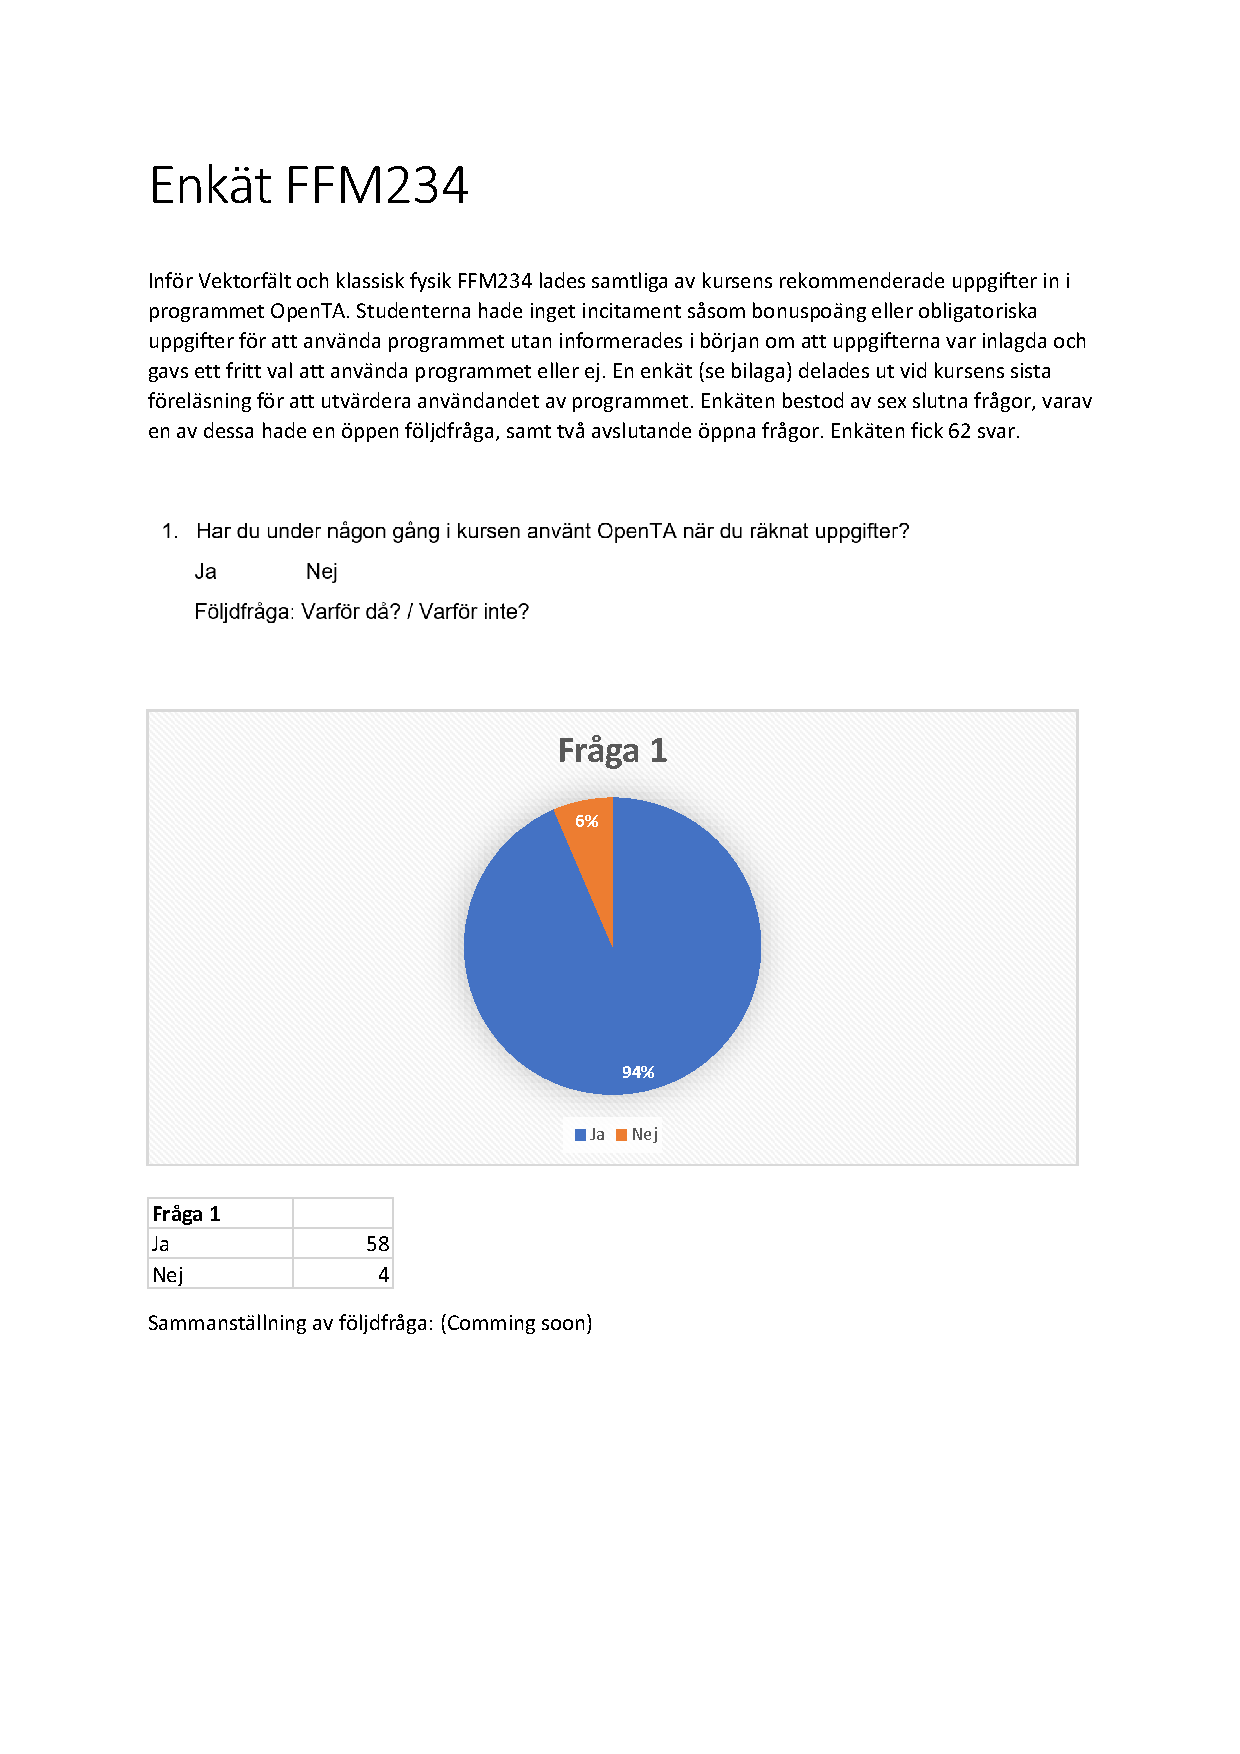
\includegraphics[page=1,scale=0.85]{appendix/form_survey.pdf}
    \caption*{Sammanställning av användarstudie (OpenTA, kurs FFM234), Sida 1}
    \label{fig:openform1}
\end{figure}


\begin{figure}[hbtp]
    \centering
    \includegraphics[page=2,scale=0.85]{appendix/form_survey.pdf}
    \caption*{Sammanställning av användarstudie (OpenTA, kurs FFM234), Sida 2}
    \label{fig:openform2}
\end{figure}


\begin{figure}[hbtp]
    \centering
    \includegraphics[page=3,scale=0.85]{appendix/form_survey.pdf}
    \caption*{Sammanställning av användarstudie (OpenTA, kurs FFM234), Sida 3}
    \label{fig:openform3}
\end{figure}

\begin{figure}[hbtp]
    \centering
    \includegraphics[page=4,scale=0.85]{appendix/form_survey.pdf}
    \caption*{Sammanställning av användarstudie (OpenTA, kurs FFM234), Sida 4}
    \label{fig:openform4}
\end{figure}

\begin{figure}[hbtp]
    \centering
    \includegraphics[page=5,scale=0.85]{appendix/form_survey.pdf}
    \caption*{Sammanställning av användarstudie (OpenTA, kurs FFM234), Sida 5}
    \label{fig:openform5}
\end{figure}

\begin{figure}[hbtp]
    \centering
    \includegraphics[page=6,scale=0.85]{appendix/form_survey.pdf}
    \caption*{Sammanställning av användarstudie (OpenTA, kurs FFM234), Sida 6}
    \label{fig:openfor6}
\end{figure}

\section{KJ-analys av användarstudie}
\label{app:kjOpenTA}

KJ-analys bygger på att samla flera människors perspektiv av samma information för att tillsammans få en bättre bild av det analyserade materialet \cite{kj}. I detta specifika fallet sammanställdes resultaten av användarstudien och analyserades med hjälp av KJ-analys kring frågorna ''Varför har du använt OpenTA?'', ''Vad har varit bra?'' och ''Vad har du saknat?''. Resultatet av analysen representeras grafiskt nedan i form av en illustration för varje fråga. På grund av storleken av illustrationerna har den roterats och delats upp i flera delar. 

% Figure Blue nr1

\begin{figure}[hbtp]
    \centering
    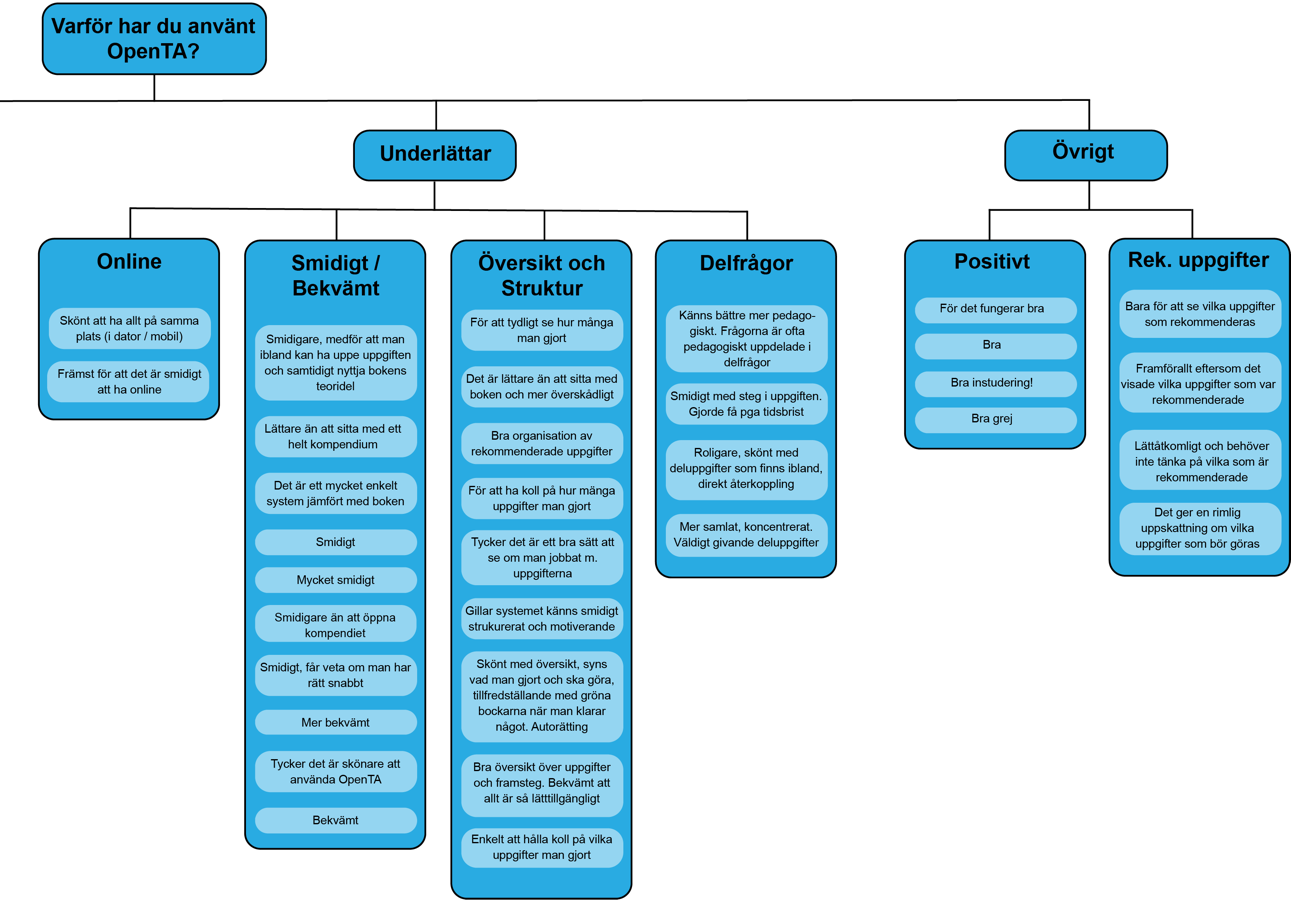
\includegraphics[scale=0.50,angle=90]{appendix/appendix_blue/nr1_part2.png}
    \caption*{}
    \label{fig:nr1_part2}
\end{figure}

\begin{figure}[hbtp]
    \centering
    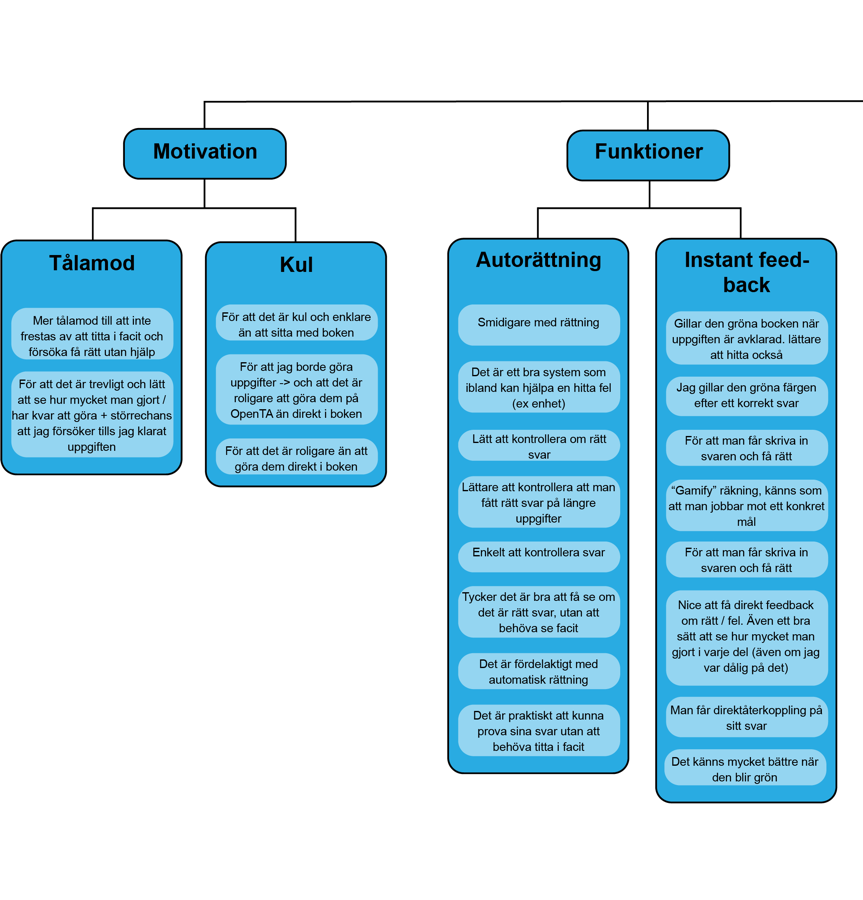
\includegraphics[scale=0.5,angle=90]{appendix/appendix_blue/nr1_part1.png}
    \caption*{}
    \label{fig:nr1_part1}
\end{figure}

% Figure blue nr7

\begin{figure}[hbtp]
    \centering
    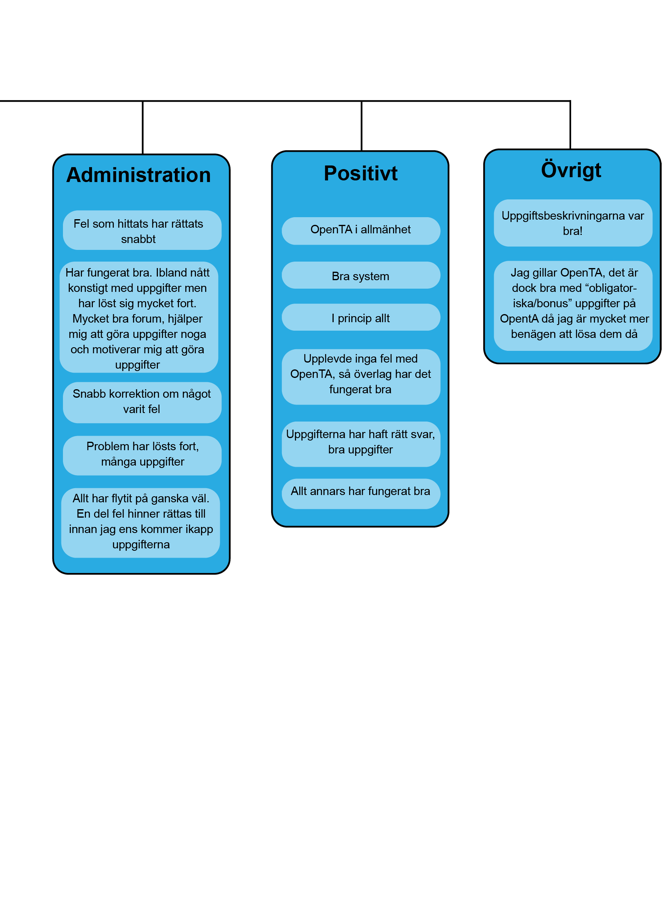
\includegraphics[scale=0.56,angle=90]{appendix/appendix_blue/nr7_part3.png}
    \caption*{}
    \label{fig:nr7_part3}
\end{figure}

\begin{figure}[hbtp]
    \centering
    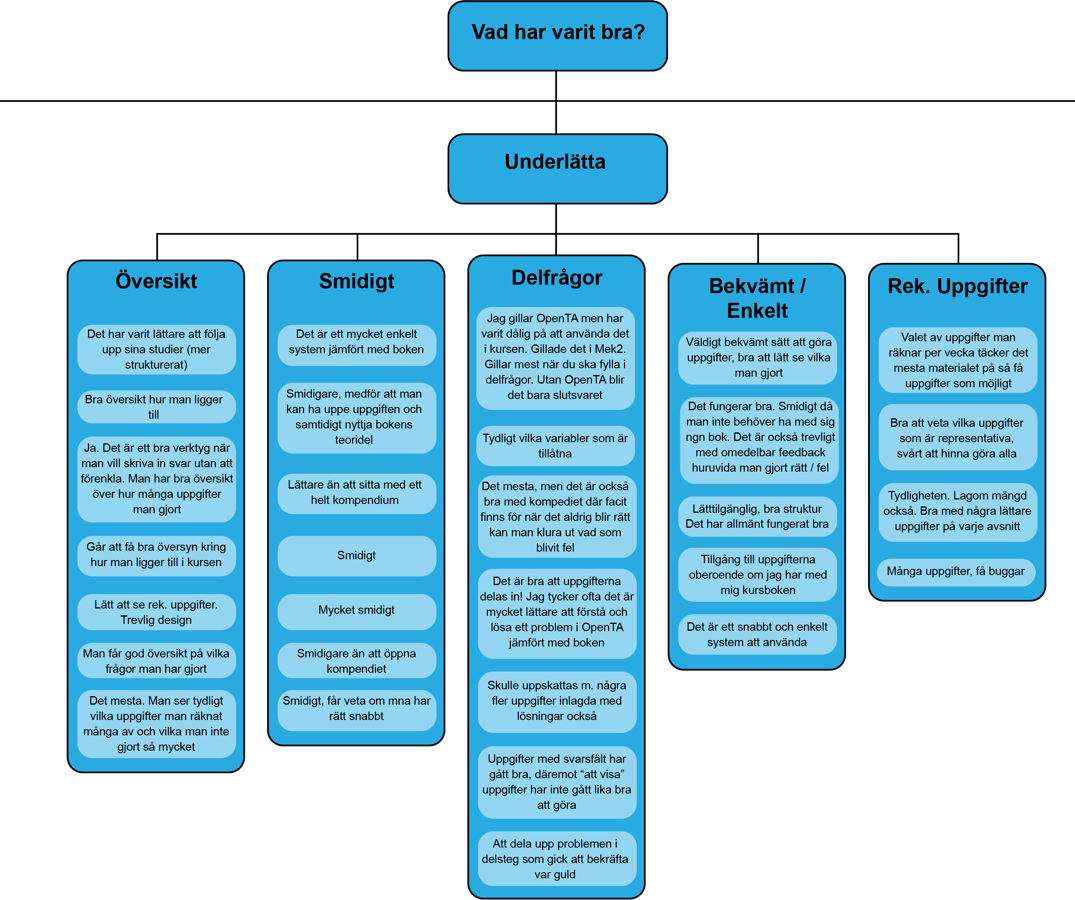
\includegraphics[scale=0.56,angle=90]{appendix/appendix_blue/nr7_part2.png}
    \caption*{}
    \label{fig:nr7_part2}
\end{figure}

\begin{figure}[hbtp]
    \centering
    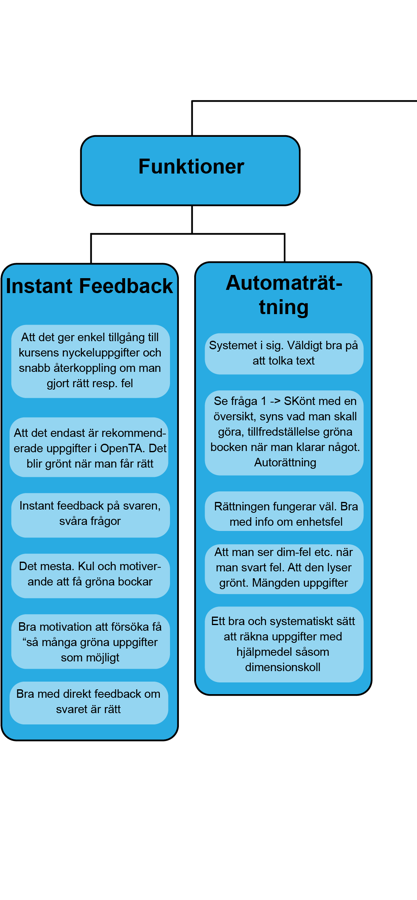
\includegraphics[scale=0.56,angle=90]{appendix/appendix_blue/nr7_part1.png}
    \caption*{}
    \label{fig:nr7_part1}
\end{figure}

% Figure blue nr8

\begin{figure}[hbtp]
    \centering
    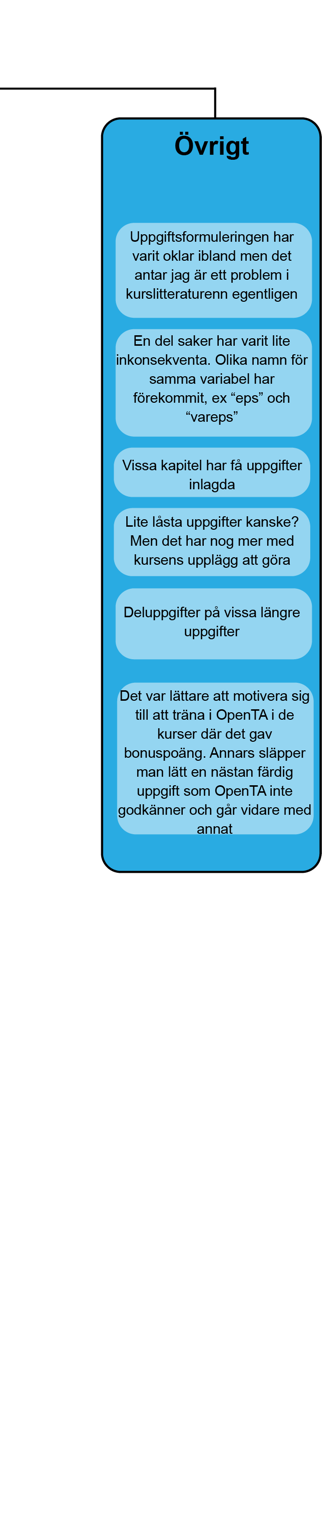
\includegraphics[scale=0.454,angle=90]{appendix/appendix_blue/nr8_part3.png}
    \caption*{}
    \label{fig:nr8_part3}
\end{figure}

\begin{figure}[hbtp]
    \centering
    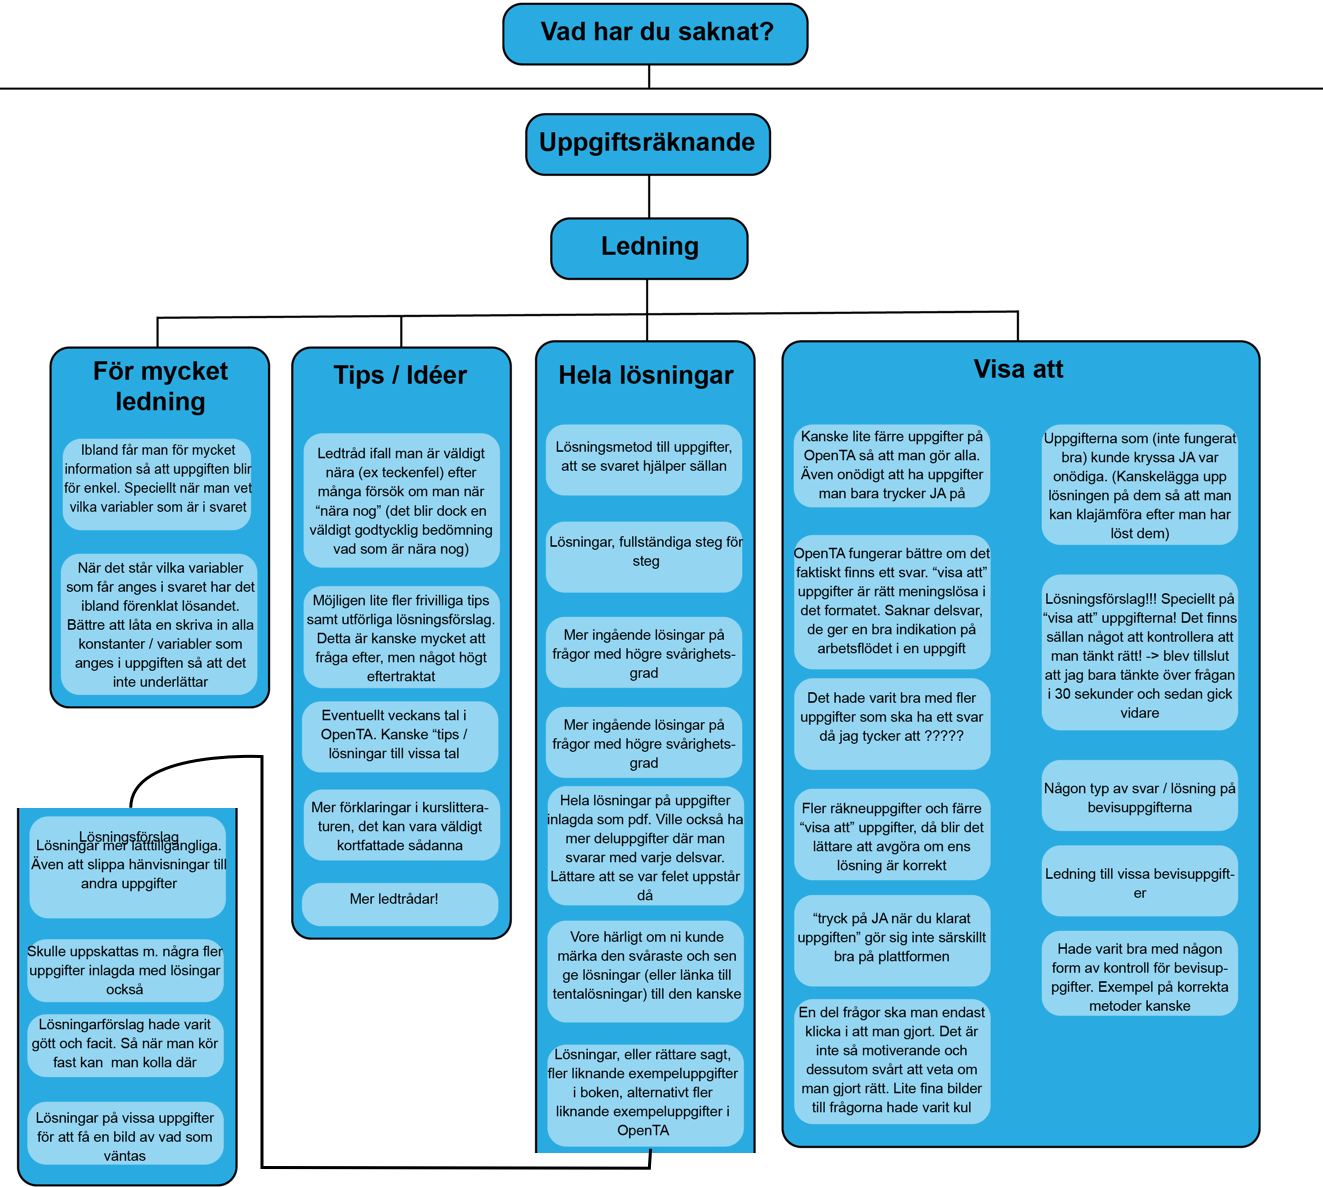
\includegraphics[scale=0.454,angle=90]{appendix/appendix_blue/nr8_part2_new.png}
    \caption*{}
    \label{fig:nr8_part2}
\end{figure}

\begin{figure}[hbtp]
    \centering
    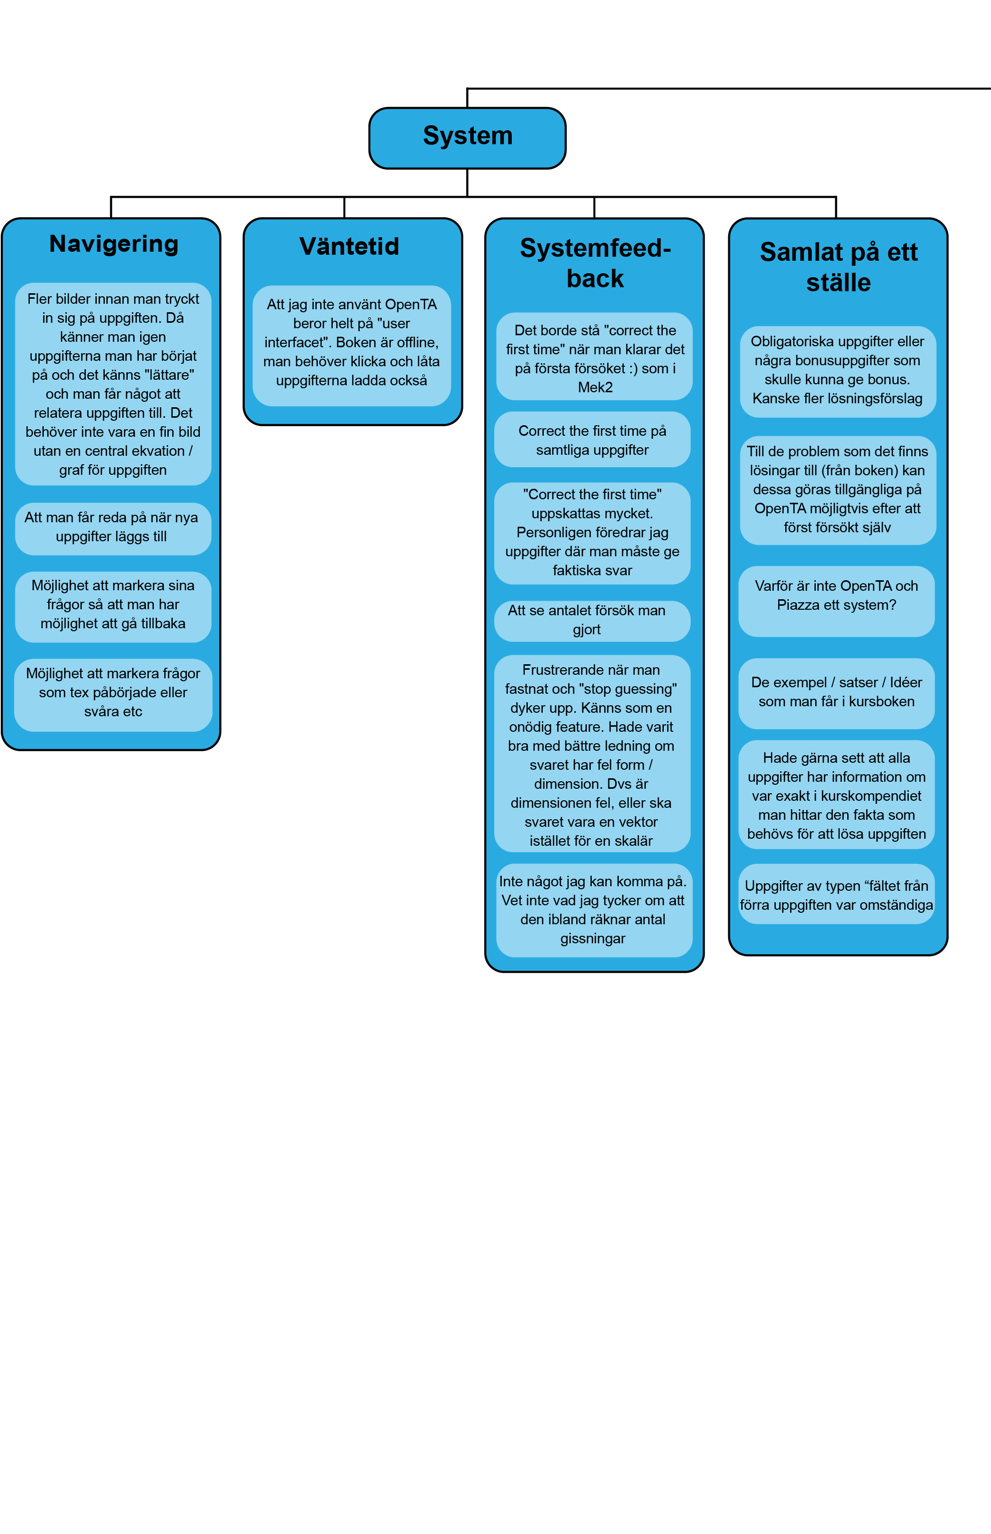
\includegraphics[scale=0.454,angle=90]{appendix/appendix_blue/nr8_part1.png}
    \caption*{}
    \label{fig:nr8_part1}
\end{figure}


%\section{Analys av syftesformuleringen}
%I sektion \ref{sec:purpose_and_problem} presenteras arbetets syftesformulering. Specifikt vill vi problematisera kring formuleringen ’’förbättrar studenters potential att lära och lärares förmåga att undervisa’’. Vi anser att begreppet förbättra inte är väldefinierat i arbetet. Formuleringen att ’’förbättra studenters potential att lära’’ kan tolkas utifrån flera perspektiv. Till exempel att studenter lär sig med en djupare förståelse, snabbare eller med mindre stress. Liknande kan formuleringen ’’förbättra […] lärares förmåga att undervisa’’ innehålla tolkningar som en minskad arbetsbelastning och möjligheter till rättvisare bedömningar av studenterna. Vår tolkning inom arbetets kontext av begreppet förbättra är att begreppet förbättra innehåller olika dimensioner såsom djupare förståelse, snabbare inlärning och mindre arbetsbelastning. Dimensionerna utgör olika frihetsgrader som kan motsäga varandra och kan därför behöva optimeras. I vidare arbete är det härav nödvändigt att vara medveten om de olika dimensionerna för att sammanlagt arbeta mot en gemensam förbättring.